\documentclass{article}

\usepackage[T1]{fontenc}
\usepackage{graphicx}
\usepackage{fancyhdr}
\pagestyle{fancy}
\fancyhf{}
\lhead{Draft 0.1}
\rhead{Elliot Oram}
\rfoot{\thepage}


\title{Video Processor Class Diagram}
\author{elo9@aber.ac.uk}

\begin{document}

\maketitle
\tableofcontents

\newpage

\section{Video Processor Class Diagram}
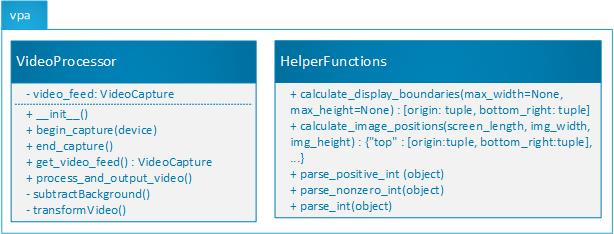
\includegraphics[width=200pt]{VideoProcessorClassDiagramImage}


\section{Description of Class Diagram}
The video processing will be performed by a single class, the \textbf{VideoProcessor}. The justification for doing this in a single class, is to remove the possibility that the video object will have to passed between classes. In addition the functionality required for video feed manipulation doesn't have many stages so can be easily represented as functions in a single class.

\begin{itemize}

	\item \textbf{Video}: The video variable is of type Video. This class type holds a video stream and can be imported from OpenCV. If this class can handle a live video stream, needs to be investigated with spike work. To maximise the performance of the system, and therefore the speed of processing, the video object may be treated as a global object (meaning it does not get passed into and out of functions). To allow for the preferred private video variable, investigation into the representation of python objects will be required. This investigation will aim to discover if references or pointer to objects can be passed between functions, rather than the full object itself.

	\item \textbf{subtractBackground}: The subtractBackground function will be used to ensure that only the Actor is shown in the video feed and the background is removed (set to black (RGB(0,0,0)). Based on research stated in the Outline Project Specification, This will use simple background subtraction or moving average background subtraction. Spike solutions will be carried out during the creation of the prototype to assess if the image processing machine is capable of more complex background subtraction techniques. Furthermore, it will test if simple background subtraction techniques produce the required effect.

	\item \textbf{transformVideo}: The transformVideo function will duplicate the video feed into 4 identical. The feeds are rotated by 90 from one another around the centre of the display monitor.This is the format that is expected for the pyramid to produce holograms.

	\item \textbf{outputVideo}: The outputVideo function will add the video feed to a window and this will be displayed on the monitor in the Viewing Area to create the hologram.

\end{itemize}

\end{document}